\documentclass[12pt]{article}

\usepackage{amsmath,amssymb, amsbsy}    % need for subequations
\usepackage{graphicx}   % need for figures
\usepackage{verbatim}   % useful for program listings
\usepackage{color}      % use if color is used in text
\usepackage{subfigure}  % use for side-by-side figures
\usepackage{hyperref}   % use for hypertext links, including those to external documents and URLs
\usepackage{bbm}
\usepackage{booktabs}

\newcommand\givenbase[1][]{\:#1\lvert\:}
\let\given\givenbase
\newcommand\sgiven{\givenbase[\delimsize]}

\begin{comment}
\pagestyle{empty} % use if page numbers not wanted
\end{comment}



\begin{document}

\section{Notes}
\subsection{Errata}
Some side notes on the supplementary material:

 \hspace*{-35pt}
\begin{small}
https://www.biorxiv.org/content/biorxiv/suppl/2018/10/01/431957.DC1/431957-1.pdf
\end{small}
I start page numbering from page 15 out of 30 of the above-mentioned document. Hence page 1 starts with the section `Materials and Methods', subesection `Gene selection'.


\begin{itemize}
   \item Page 1, paragraph 4, line 2 and line 4: is $s[\mathbb{G}] $ meant to be  $S[\mathbb{G}] $?
   \item Page 8, paragraph 1, line 3 from the end of the paragraph: $\Lambda x \sim Gamma (x; r,\frac{\beta}{\Lambda})$. I would rewrite that as $\Lambda x \sim Gamma (r,\frac{\beta}{\Lambda})$, ie. ommit $x$. (This is also repeated elsewhere in the document). Also very srtictly speaking $x$ is a random variable and $\Lambda$ just a parameter which is assumed known, hence $x$ should probably be $X$ and  $\Lambda$ just $\lambda$. But since this is not a mathematics paper and for the shake of simplicity using small letters to denote both a random variable and an observed value, depending on the context, should probably be fine.
   \item  Page 8, paragraph 1, last line. I would explicitly add the conditionals:
	$\left.
     		\begin{tabular}{lll}
       		$x \given \lambda \sim Poisson(\lambda)$ \\
       		$\lambda \given r, \mu \sim \Gamma(r, \frac{r}{\mu})$ \\
     		\end{tabular}
   	\right\}  x \given  r, \mu \sim NB(r, \mu) $

    \item Page 9, paragraph 1, line 2 and line 3. I think $r_0$ is $\bar{r}$ 
    \item Page 9, paragraph 1, line 3. I understand the phrase `normalised Gaussian density of radius $r_0$' as bivariate gaussian density with zero correlation, mean ${\bf x}_c$ and the same standard deviation across its two dimensions, denoted by $r_0$
    \item Page 9, bottom of the page, in the likelihood equation, I think we should replace $ = $ with $\propto$
    \item Page 10, lines 9-10 from the bottom: `expected efficiency $\eta_0$'. Something looks strange here, for example $\eta_0$ is not the expectation of the gamma-distributed $\eta_g$.
    \item Page 10, bottom of the page, equation of the joint log-density: I might show how this can be broken up (assuming independence between $\zeta, \gamma $ and $\eta$):
	\begin{align}
		\text{p}({\bf x}, g, z, \zeta, \gamma, \eta) & =  \text{p}({\bf x}, g, z \given \zeta, \gamma, \eta) \, \text{p}(\zeta, \gamma, \eta) \nonumber\\
							      & =\text{p}({\bf x}, g, z \given \zeta, \gamma, \eta) \, \text{p}(\zeta) \, \text{p}(\gamma) \, \text{p}(\eta) \nonumber
	\end{align}
     \item Page 10, bottom of the page, equation of the joint log-density: \[\sum_{g,c}\log Gamma(\gamma_{g,c} \given r, r) \text{ and} \sum_{g,c}\log Gamma(\eta_g \given r, r/\eta_0)\]
Move conditioning symbol inside the parentheses, at the end, ie:
 \[\sum_{g,c}\log Gamma(\gamma_{g,c}, r  \given r) \text{ and} \sum_{g,c}\log Gamma(\eta_g, r/\eta_0 \given r)\]

     \item Page 11, equation (1), some point as above.

     \item Page 11,  lines 8 and 9 from the bottom: $N_{c,g}$ needs its subscripts swapped I think, ie it should be: $N_{g,c}$.  The latter is the notation used in the rest of the paper.

    \item Page 11, line 2 from the bottom of the page: `we could integrate $\int q(\gamma \given \zeta) d\gamma$' is probably meant to be `we could integrate $q(\gamma, \zeta)$ over $\gamma$'

    \item Page 12, last two lines of the page: Something is wrong with the reference. There is an error that the reference source is not found.

   \item Page 14. In the pseudocode, in the main loop, compute step number 4: Again, reference source is not found. 

   \item General comment. I would explicitly add/state that $x$ denotes counts whereas ${\bf x}$ locations. Sometimes also, (and I might sound excessively pedantic here...) ${\bf x}$ and  $\textit{\textbf{x}}$ are used interchangeably (page 9, log-density and page 10, intensity function).

   \item I might be wrong but I am a bit a bit puzzled about the expected gamma expression in the Matlab code. For example line 135 of \texttt{call\_cell.m}, shouldnt the nominator and denominator be the other way round? See  figure \ref{fig:eSpotGamma}

\begin{figure}[!ht]
  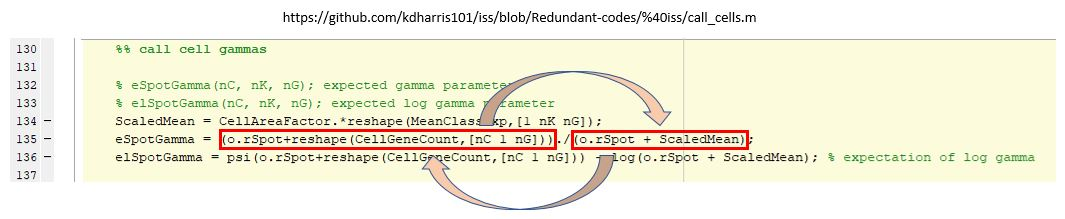
\includegraphics[width=\linewidth]{eSpotGamma.jpg}
  \caption{Code snip.}
  \label{fig:eSpotGamma}
\end{figure}



\end{itemize}
\end{document}